\documentclass[tikz,border=3mm]{standalone}
% общий стиль (подключается через TEXINPUTS)
% tikz-style.tex (общий стиль для всех TikZ-картинок)
\RequirePackage[T1,T2A]{fontenc}
\RequirePackage[utf8]{inputenc}

% Palatino-подобный шрифт (как в MathJax часто воспринимается «более вытянутым»)
\RequirePackage{txfonts}
% txfonts даёт предупреждение по кириллице (T2A/txr не определён).
% Оставляем txfonts для математики, а текстовый шрифт возвращаем на Computer Modern,
% чтобы не искать T2A/txr и убрать предупреждения.
\renewcommand{\rmdefault}{cmr}
\renewcommand{\sfdefault}{cmss}
\renewcommand{\ttdefault}{cmtt}

\RequirePackage{tikz}
\RequirePackage{xcolor}
\usetikzlibrary{calc}

% цвета
\definecolor{lightgreen}{RGB}{214,234,214}
\definecolor{darkgreen}{HTML}{0B7A0B}
\definecolor{darkred}{HTML}{DF0000}

\definecolor{midgreen}{HTML}{2E9B2E}
\definecolor{palegreen}{RGB}{235,246,235}
\definecolor{olivegreen}{HTML}{3E6B2F}

\definecolor{lightred}{RGB}{255,220,220}
\definecolor{midred}{HTML}{E04545}
\definecolor{darkred2}{HTML}{A80000}

\definecolor{lightblue}{RGB}{220,232,255}
\definecolor{midblue}{HTML}{2E5BD6}
\definecolor{darkblue}{HTML}{0B2E8A}

\definecolor{lightgray}{RGB}{240,240,240}
\definecolor{midgray}{RGB}{170,170,170}
\definecolor{darkgray}{RGB}{80,80,80}

\definecolor{vtxfill}{RGB}{86,193,255}
\definecolor{vennfill}{RGB}{220,232,255}


% единый набор стилей TikZ
\tikzset{
    lab/.style={
        font=\fontsize{24}{32}\selectfont
    }
}

\usetikzlibrary{matrix,decorations.pathreplacing,positioning}
\newcommand{\digitfont}{\ttfamily\Large}

\begin{document}
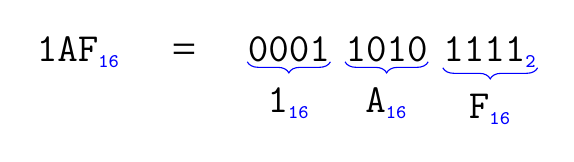
\begin{tikzpicture}[font=\rmfamily\Large]
\node (left) {{\digitfont 1AF\textsubscript{\textcolor{blue}{\scriptsize\ttfamily 16}}}};
\node[right=4mm of left] (eq) {$=$};
\matrix (m) [matrix of nodes, nodes={font=\digitfont, anchor=base, inner sep=0pt}, column sep=2mm, right=4mm of eq] {
0001 & 1010 & 1111\textsubscript{\textcolor{blue}{\scriptsize\ttfamily 2}}\\
};

\draw[decorate, decoration={brace, amplitude=4pt, mirror}, blue]
(m-1-1.south west) -- (m-1-1.south east);
\draw[decorate, decoration={brace, amplitude=4pt, mirror}, blue]
(m-1-2.south west) -- (m-1-2.south east);
\draw[decorate, decoration={brace, amplitude=4pt, mirror}, blue]
(m-1-3.south west) -- (m-1-3.south east);

\node[below=6pt of m-1-1] {{\digitfont 1\textsubscript{\textcolor{blue}{\scriptsize\ttfamily 16}}}};
\node[below=6pt of m-1-2] {{\digitfont A\textsubscript{\textcolor{blue}{\scriptsize\ttfamily 16}}}};
\node[below=6pt of m-1-3] {{\digitfont F\textsubscript{\textcolor{blue}{\scriptsize\ttfamily 16}}}};
\end{tikzpicture}
\end{document}
